\chapter{Results and Discussion}

\section{Dataset}

\subsection{Stanford Sentiment Treebank}
In this thesis, we use Standford Sentiment Treebank (SST) dataset \cite{socher2013recursive}. Standford Sentiment Treebank contains 11,855 sentences. Each data sentence consist of fined-grain sentiment labeled phrases in constituency parse tree structure (see \textbf{Figure \ref{fig:sst}}). There are total 215,154 phrases in whole dataset.
The dataset was splitted into train/dev/test contain 8544/1101/2210 sentences each for training and evaluation models. After remove neutral sentiment sentences, there are 6920/872/1821 sentences remained in train/dev/test set.

SST dataset are publicly available online \footnote{https://nlp.stanford.edu/sentiment/index.html}.

\begin{figure}[H]
	\begin{minipage}{\textwidth}
		\centering
		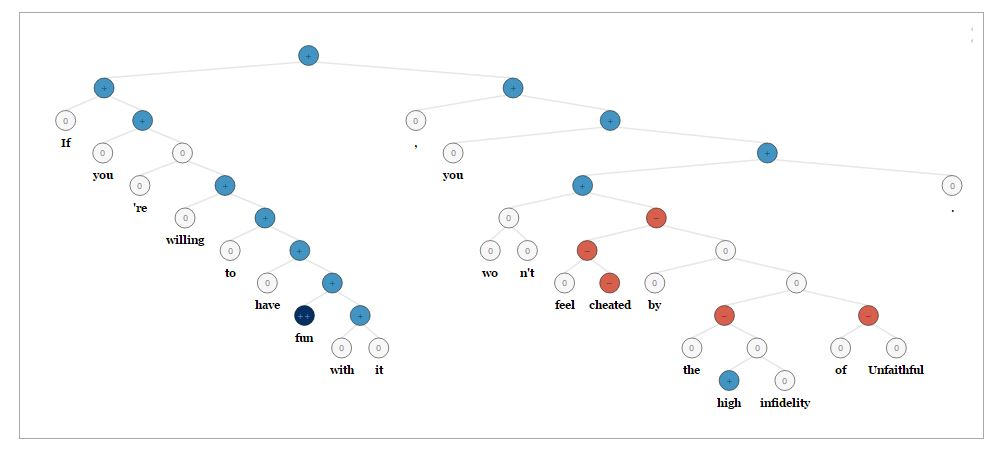
\includegraphics[width=0.9\linewidth]{figure/sst}
		\caption[A parsed sentence in SST]{A parsed sentence in SST \footnote{Render by Pytreebank \url{https://github.com/JonathanRaiman/pytreebank}}}
		\label{fig:sst}
	\end{minipage}
\end{figure}

\subsubsection{Preprocess}
We use preprocess source code from \cite{socher2013recursive} implementation \footnote{\url{https://github.com/stanfordnlp/treelstm}} to preprocess SST.



\subsection{Amazon Movies Review}
We get Amazon Movies and TV reviews (4,607,047 reviews) and Amazon Book reviews (22,507,155 reviews) \cite{he2016ups}. Listing \ref{lst:amzrevie} is sample of one book review.

\begin{lstlisting}[caption={Amazon reviews sample},label={lst:amzreview}]
	{
		"reviewerID": "AH2L9G3DQHHAJ",
		"asin": "0000000116",
		"reviewerName": "chris",
		"helpful": [5, 5],
		"reviewText": "Interesting Grisham tale of a lawyer that takes millions of dollars from his firm after faking his own death. Grisham usually is able to hook his readers early and ,in this case, doesn't play his hand to soon. The usually reliable Frank Mueller makes this story even an even better bet on Audiobook.",
		"overall": 4.0,
		"summary": "Show me the money!",
		"unixReviewTime": 1019865600,
		"reviewTime": "04 27, 2002"
	}
\end{lstlisting}

\subsubsection{Preprocess}
\textbf{Step 1:}
We extract reviewText and overall from review dataset. We assume that overall valus are sentiment score for reviews. Reviews with overall 5 is very positive and 0 is very negative. We keep asin, reviewText, overall and ommit other data points.

\textbf{Step 2:}
We group dataset by product (reviews with same asin). Then for each product, we sorted by overal.

\textbf{Step 3:}
We dump all reviewText into plain text file. We preprocess Standford Tokenizer \cite{tokenizerpart}.

We also make a version of unsorted dataset. We preprocess as we do to our sorted dataset. However, in \textbf{Step 2:}, instead sort review, we suffle all reviews.

% how to preprocess amazon movies reviews

\subsubsection{Train Glove on Amazon Review dataset}
We train our word representation from Amazon dataset using Glove \cite{pennington2014glove} on 15 iteration with windows size of 20.





\section{Evaluation}


% Please add the following required packages to your document preamble:
% \usepackage{booktabs}
% Please add the following required packages to your document preamble:
% \usepackage{booktabs}
\begin{table}[]
	\centering
	\caption{My caption}
	\label{my-label}
	\begin{tabular}{@{}lll@{}}
		\toprule
		& Constituency Tree-LSTM & LSTM \\ \midrule
		Glove 42B             &                        &      \\
		Glove 840B            &                        &      \\
		Glove (Amazon)        &  88.45           &      \\
		Glove (Amazon Sorted) &  88.85           &      \\
		Paragram-Phrase XXL   &                        &      \\
		SSWEu                 &                        &      \\ \bottomrule
	\end{tabular}
\end{table}
